% file: reasoning_case.tex

\begin{ReasoningBox}[title=Temporal Relation Reasoning] % 可以通过 title 参数修改标题
    % --- 第一部分：问题描述与图片 ---
    % \begin{minipage}[t]{0.58\textwidth}
    
        \textbf{Question:} Based on the provided 'GoldSteinScale' time series and event timestamps, determine the correct chronological order of the following events:
    \\
    (1) The Australian Manufacturing Workers' Union, Australian Workers' Union, and Electrical Trades Union are involved in industrial action against Qantas, targeting the airline's engineers to demand better wages and working conditions \ldots
    \\
    \begin{wrapfigure}{r}{0.6\textwidth}
        \centering
        % wrapfigure 通常顶部会有多余空白，使用负 vspace 向上提，让图片和第一行文字对齐
        \vspace{-20pt} 
        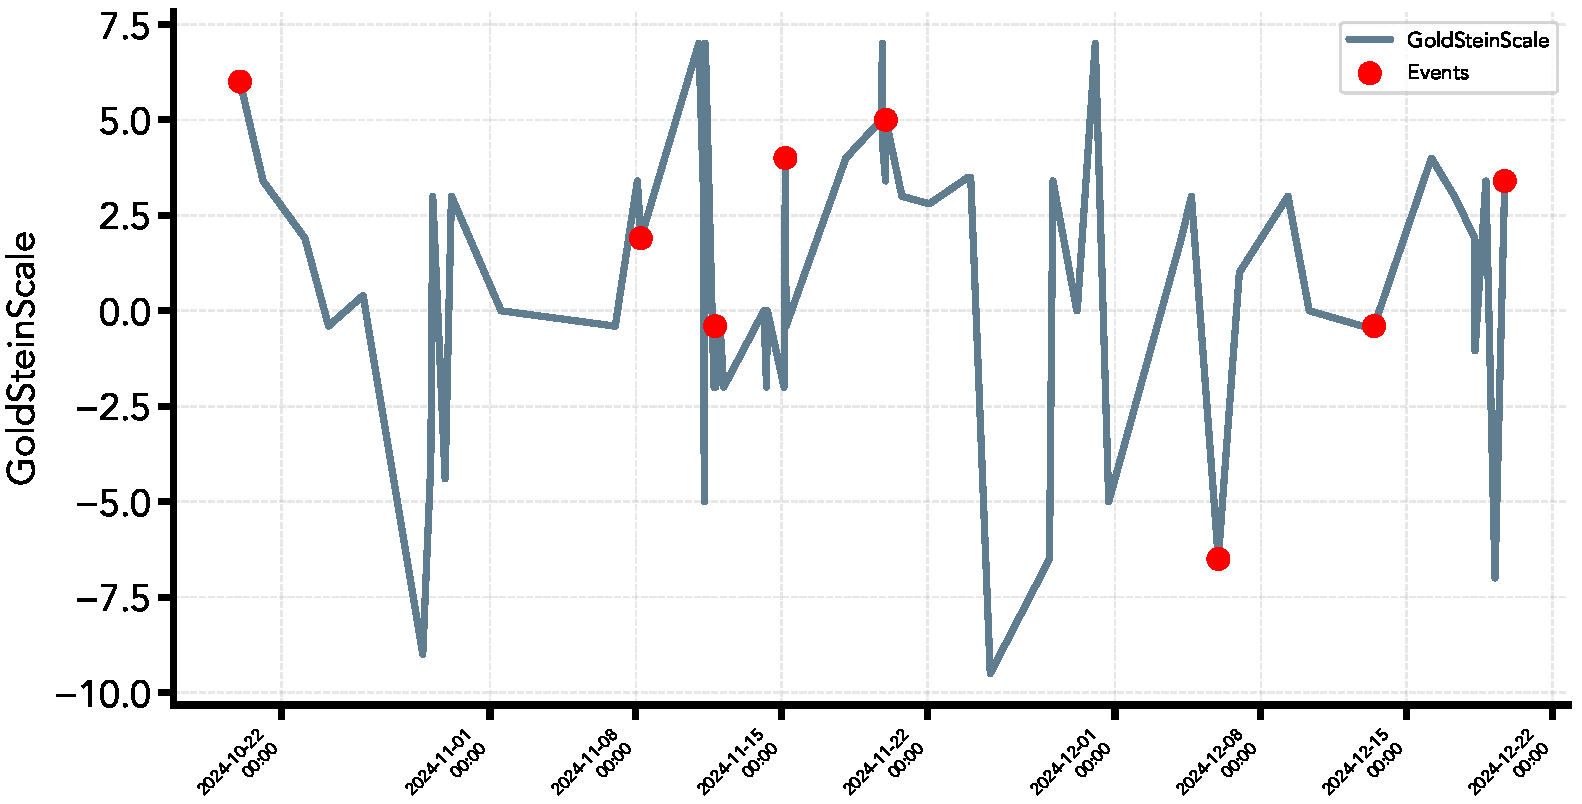
\includegraphics[width=\linewidth]{blocks/sample_cases_success/temporal.pdf}
        % 调整底部的留白
        \vspace{-20pt}
    \end{wrapfigure}
    (2) The article does not directly mention labor unions or their activities. It highlights how Australian workers are increasingly using AI and robotics to reduce monotonous and physically demanding tasks, potentially leading to shifts in job roles and productivity. \ldots
    \\
    (3) The Australian Workers' Union (AWU) raised safety concerns prior to the incident at the Golden Plains Wind Farm, highlighting issues such as poor safety standards, non-unionized contractors, and near misses. AWU representatives expressed dissatisfaction with the company's response during a meeting, feeling their concerns were dismissed and that safety standards in the renewable sector lag behind civil construction \ldots
    \\
    (4) The Australian Manufacturing Workers' Union (AMWU) commissioned a report highlighting that reducing Australia's industrial gas use would protect jobs and support manufacturing sectors, emphasizing the importance of supporting workers through a transition to electrification and green hydrogen. AMWU's national secretary, Steve Murphy, stressed the need to prioritize gas resources for industries that employ hundreds of thousands of workers, as part of a fair industrial transition amid decarbonization efforts \ldots
    \\
    (5) Greater Victoria Canada Post workers, represented by the Canadian Union of Postal Workers (CUPW), are preparing for a potential strike after over a year of negotiations with Canada Post. The union, which includes 600 workers in the region, has voted overwhelmingly in favor of strike action, demanding a 22\% wage increase over four years and other improvements such as pensionable hours and a guaranteed 40-hour work week \ldots
    \\
    (6) The article highlights concerns from the Australian Workers' Union NSW branch secretary Tony Callinan, who emphasizes that forestry workers are "extremely worried" about their future jobs due to the potential establishment of the Great Koala National Park. Workers fear job losses in the forestry and timber processing industries if the park's creation leads to restricted wood supply and mill closures \ldots
    \\
    (7) The Australian Workers' Union (AWU) has proposed a reform for long service leave, advocating for a "portable" long service leave system that would allow workers to accumulate two months of leave over ten years working across multiple employers. The union, representing 75,000 members, urged the federal government to implement this change, emphasizing its benefits for workers in insecure employment, such as casuals \ldots
    \\
    (8) The article highlights industry advocacy by the Victorian Automotive Chamber of Commerce (VACC) and the Motor Trades Association of Australia (MTAA), which are representative organizations akin to labor unions. These groups supported the inclusion of automotive trades on the revised Core Skills Occupation List (CSOL) to address labor shortages, emphasizing the importance of skilled migration for workforce solutions. They submitted evidence-backed data to the government, demonstrating the critical need for skilled automotive workers. \ldots

\noindent \textbf{Event Timestamps (random order):}
\begin{itemize}
    \item 2024-12-13 10:30:00
    \item 2024-12-19 17:00:00
    \item 2024-11-11 19:15:00
    \item 2024-11-15 04:15:00
    \item 2024-12-05 23:00:00
    \item 2024-11-08 05:45:00
    \item 2024-11-20 00:00:00
    \item 2024-10-20 00:00:00
\end{itemize}
    \vspace{0.5em}
    % --- 第二部分：选项 ---
    \textbf{Answer Choices:} \\ (A) (2)(6)(4)(7)(8)(3)(5)(1) \\ (B) (2)(5)(3)(7)(4)(8)(6)(1) \\ (C) (4)(8)(2)(6)(1)(7)(5)(3) \\ (D) (4)(3)(6)(5)(1)(2)(8)(7) \\
    \textbf{Correct Answer:} \textcolor{correctgreen}{(B)} \\
\end{ReasoningBox}